\subsection{Hager Group}

Hager Group se positionne en tant que leader mondial dans le domaine des solutions pour les installations électriques dans les secteurs résidentiels, tertiaires et industriels. En offrant une gamme complète, de la distribution d'énergie à la gestion intelligente des bâtiments, en passant par le cheminement de câbles et les dispositifs de sécurité, l'entreprise incarne l'innovation électrique. Dirigée de manière indépendante par les membres de la famille Hager, elle opère depuis son siège à Blieskastel, en Allemagne. Avec 13 000 collaborateurs répartis sur 22 sites dans le monde, Hager Group réalise un chiffre d'affaires de 3,1 milliards d'euros (2023) et exporte ses solutions vers plus de 100 pays. La confiance mondiale témoignée envers Hager Group est le socle de son succès continu.

\subsection{Résumé du projet}

L'objectif principal de ce projet est de concevoir une architecture de type GAN afin d'étendre la base de données du groupe Hager, avec pour finalité d'améliorer la détection des défauts d'arc au sein de leurs installations. Ces données synthétiques seront générées à partir d'une base de données réelle et volumineuse fournie par Hager.

\subsection{GAN}

Les réseaux génératifs antagonistes (GAN) sont une catégorie de modèles d'apprentissage profond extrêmement novateurs. Les GAN, composés d'un générateur et d'un discriminateur, ont été développés dans le but de générer des données synthétiques qui ne sont pas distinguables des données réelles. 


\begin{figure}[h]
    \centering
    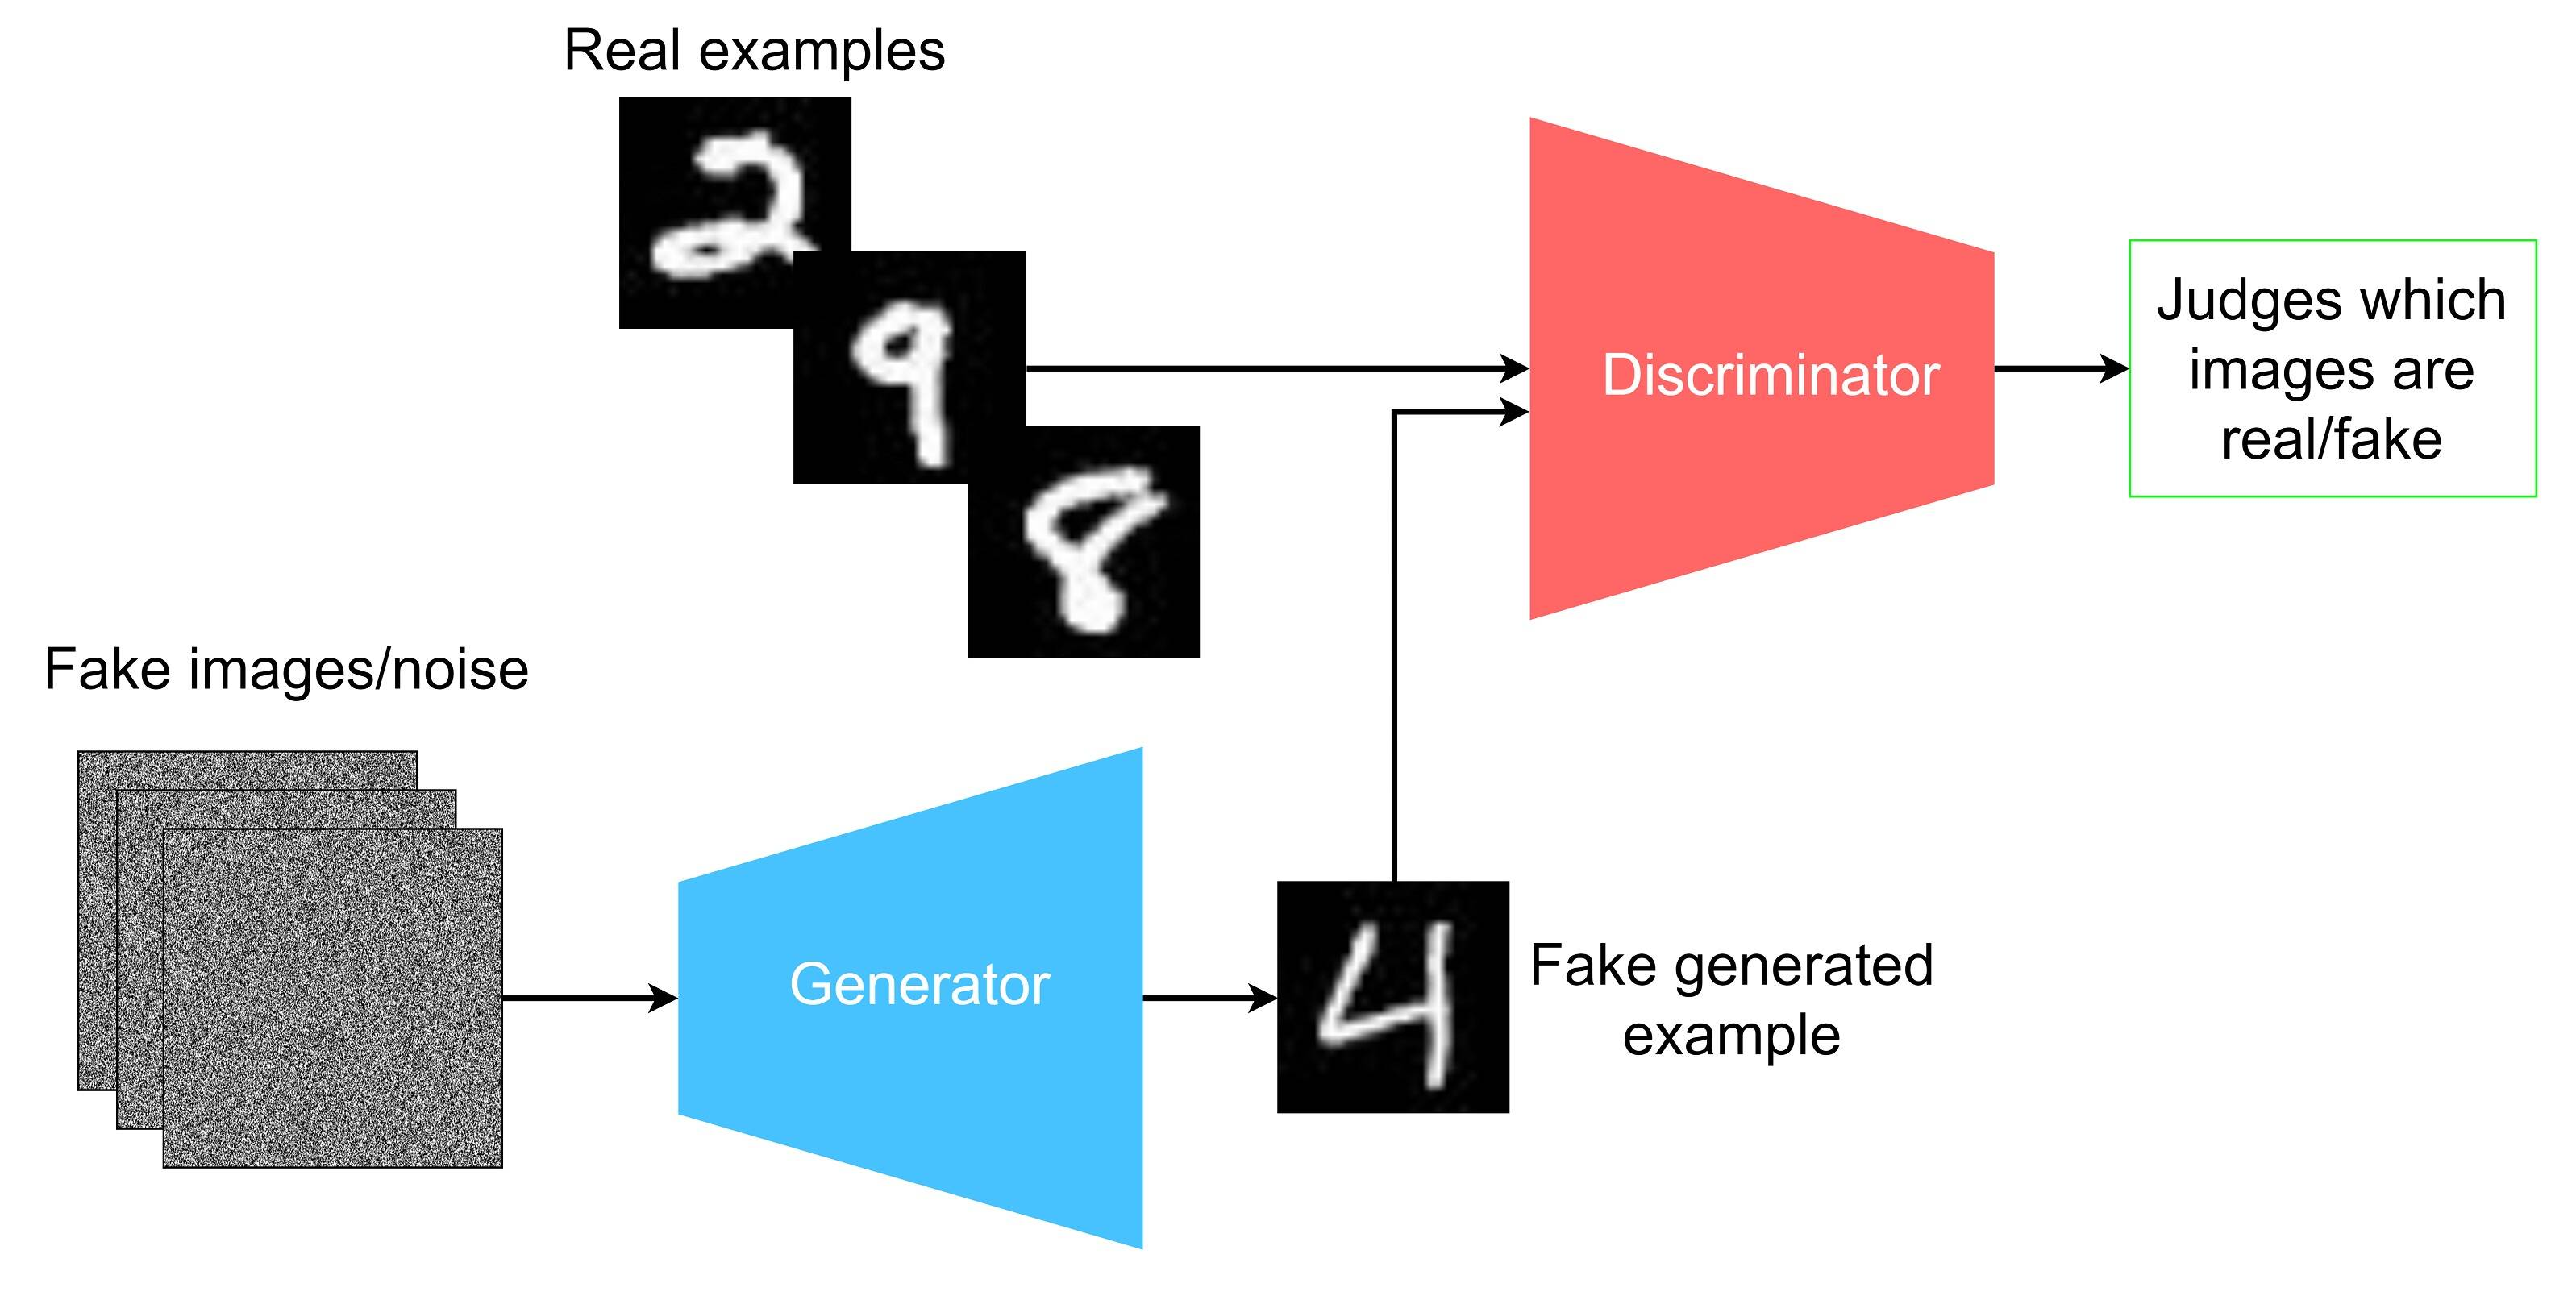
\includegraphics[width=0.6\textwidth]{logos/GANs.jpg}
    \caption{Fonctionnement imagé d'un GAN}
\end{figure}
